\chapter{相关技术研究}
随着互联网技术的发展与国民生活水平的提供,手机持有率也直线上升,
这使得手机网民大规模的增长,人们在网上产生的信息、发布的文本日益碎片化。
为了有效利用这些片段化的信息,短文本分类技术,作为自然语言处理的关键技术之一,也得到了充分的关注与发展,
短文本分类应用的影子在互联网中随处可见。
本章将对传统文本分类技术进行论述,并介绍本文涉及到的相关技术问题。
\section{中文文本分词}
词是最小的能够独立活动的有意义的语言成分,在英文文本中,每个单词天然的由空格分割开来,
使得研究人员可以毫无难度的获取文本中所有的单词,然后进行接下来的研究工作。
但对于中文这样由字组成的连续文本,不存在这样的语言优势,词语直接没有明确的区分标记,
要想进行语义分析,必须先将中文文本切分,因此中文分词是中文信息处理的基础和关键。
同时,大量实验表明,分词的好坏直接关系着后续分类算法的最终效果,所以选择一个快速并
准确的分词算法尤为重要。目前常用的分词方法主要有两大类:基于字符串匹配的算法,基于规则的算法。
\subsection{基于字符串匹配的分词算法}
基于字符串匹配的分词算法又称为机械分词算法,主要依据外部提供的词典,
按照一定的策略将待切分的中文文本与词典中的词条逐一匹配,
若在词典中找到该词条,则匹配成功,否则做其它相应的处理。
查找词库的匹配策略分为两种:长单词优先的最大匹配法以及短单词优先的最小匹配法。
在实际使用中,人们发现单词切分次数越短,切分出的单词越长,分词效果越好,
所以目前一般使用最大匹配法。
按照匹配顺序的不同,最大匹配算法又可分为:正向最大匹配算法\citing{张劲松2009回溯正向匹配中文分词算法}、
逆向最大匹配算法\citing{李娟2010一种改进的逆向匹配快速切分算法}、
双向最大匹配算法\citing{陈耀东2005基于有向图的双向匹配分词算法及实现}。

(1)正向最大匹配算法

正向最大匹配算法的基本思想是:已知词典中最长单词的长度为$N$,则以$N$最为截取单词初始长度。
对于带切分的中文文本$S$,首先从左向右截取长度为$N$的字符串$W_{1}$,
然后在词典中寻找是否有和该字符串$W_{1}$匹配的单词。如果找到,则将$W_{1}$标记为成功切分出的单词,
再继续从待切分文本的$N+1$处开始下一次匹配;如果没找到,则将截取长度减$1$重新截取,即在$S$的原来位置重新截取长度为$N-1$的字符串,
然后重复之前匹配操作,直到截取长度为$1$。算法流程如图\ref{max_match}所示:

\begin{figure}[h]
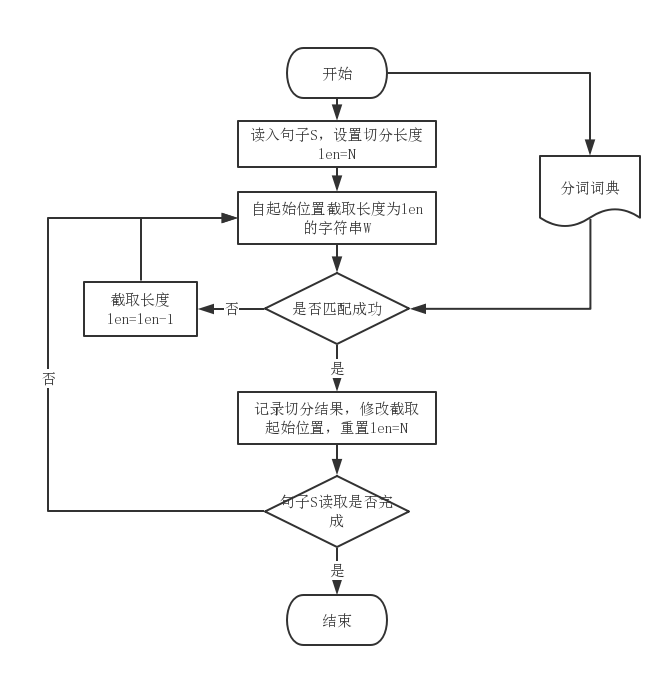
\includegraphics[scale=0.6]{picture/max_match.png}
\caption{正向最大匹配算法流程}
\label{max_match}
\end{figure}

(2)逆向最大匹配算法

逆向最大匹配算法思路和正向最大匹配算法大致相同,不同之处在于截取字符串时的方向由从左向右换成了从右向左。
也就是说,当对句子分词时,根据词典中最长单词的长度,从句子末尾开始向左截取字符串与词典中的
单词匹配,直到切分到句子的开始位置为止。

(3)双向最大匹配算法

双向最大匹配算法是上述两种最大匹配算法的结合,侧重于分词过程中的检错和纠错,其基本思路是对待分词文本分别
采用正向最大匹配和逆向最大匹配进行初步切分,然后将得到的正向分词结果和逆向分词结果进行比较,如果
两种方法的结果一致,则认为分词结果正确,如果结果存在出入,则认为分词存在着切分错误,需要采用其他技术手段消除
结果中的歧义。

从上面的分析可以明显看出,无论哪种最大匹配算法都极度依赖词典,只有在词典覆盖的领域内,才有较理想
的分词效果。对与词典没有覆盖的陌生领域语料,极端情况下甚至会出现单字切分的分词结果。

\subsection{基于统计的分词算法}

这类分词算法并不依赖具体的词典,而是根据语料中的统计信息,识别句子中的单词。即把单词看做是
特定的字的结合,在语料中邻近的字共同出现的次数越多越可能是一个词。所以计算句子中特定字的组合的出现概率,
可以判断这个组合是否是一个词。通过以概率论为理论基础,将中文文本中的每一个词的出现抽象成随机过程,
分词算法不会被待分词文本的内容所影响,对所有领域的中文语料都有统一的效果,
这是极度依赖词典的基于字符串匹配的分词算法所没有优势。根据采用的统计模型不同,基于统计的分词算法
又可分为互信息算法、N元统计模型等。

(1)互信息算法

在概率论和信息论中,两个随机变量的互信息是这两个变量彼此之间依赖性的一个度量。更确切的说,它是根据另一个
随机变量来量化从一个随机变量中可以获得的信息量。互信息分词算法是互信息理论在分词中的应用,通过计算
两个相邻字符串的互信息值,判断它们之间的结合程度。

对于两个相邻字符串$x$和$y$,它们的互信息值计算公式如下:
\begin{equation}
    I\left ( x,y \right )=\log \frac{p\left ( x,y \right )}{p\left ( x \right )p\left ( y \right )}
\end{equation}

其中$p\left ( x,y \right )$表示字符串$x$和$y$在语料中共同出现的频率,$p\left ( x \right )$与$p\left ( y \right )$分别表示字符串$x$与$y$的出现频率。
当$I\left ( x,y \right )>0$时,表示$x$和$y$具有一定的相关性,并且这个值越大,它们联系的就越紧密,
超过某一个阈值时即可判定为一个词;当$I\left ( x,y \right )=0$时,表示$x$和$y$的关系不明确;当$I\left ( x,y \right )<0$时,表示$x$和$y$直接几乎没有相关性,
基本不会组成一个词。

(2)N元统计模型

N元统计模型又称为N元语言模型(n-gram language model),本质上是对语言建模的一种统计模型。
该模型假定语言满足马尔科夫性,句子中的单词的出现与其前面出现的单词紧密相关,即第$n$个词的出现
只与前面$n-1$个词的出现相关,而和其他任何词都不相关。假设句子$S$由单词序列$\left (w_1,w_2,...,w_m  \right )$组成,
则N元语言模型可表示为:
\begin{equation}
    \begin{aligned}
        P\left ( S \right )&=P\left ( w_1w_2...w_m \right )\\
        &=P\left ( w_1 \right )P\left ( w_2|w_1 \right )...
P\left ( w_i|w_{i-n+1}...w_{i-1} \right )...P\left ( w_m|w_{m-n+1}...w_{m-1} \right )
    \end{aligned}
    \label{n-gram}
\end{equation}

理论上来说,$N$取值越大,模型就越精确,越能揭示出语言的内在结构。但随着$N$的增加,模型的计算复杂度也呈几何式上升,
所以在实际应用中,通常将$N$取值为2、3、4,而$N$取2的N元统计模型称为bigram模型,$N$取3的则称为trigram模型。

在分词应用中,算法首先对句子$S$进行全切分,得到若干分词结果,再根据公式\ref{n-gram}计算这些分词结果的概率$P\left ( S \right )$,
最后选择概率最高的分词结果作为最终结果。

\section{传统文本表示方法}
分词处理之后,文本信息转化为一个单词序列,但对于计算机与程序来说依然是一段没有意义的字符串。
为了让程序能够理解文本信息,继续之后的分类工作,我们需要对其再次处理,提取出其中的有效信息,将字符串文本
映射成结构化的数字信息。

\subsection{向量空间模型}

向量空间模型(Vector Space Model,VSM)最早由Salton等人\citing{薛苏琴2016基于向量空间模型的中文文本相似度的研究}于20世纪70年代提出,
是一种将文本信息表示为向量的代数模型。模型的主要思想是将文本看做由单词的简单组合,通过
统计语料中不同单词的个数,构建一个$n$维的向量,向量中每一个纬度都代表一个不同的单词,单词在文本中存在,则此位为$1$,否则为$0$,以此将一段文本信息
转换为一个$n$维的数学向量。

可以明显看出,虽然向量空间模型建立了一个从文本到向量的快速转换,让程序能够容易地对文本进行处理计算,
但这种映射方式太过简单。将文本表示为单词的组合,忽略了词语的位置关系以及词语之间的相互联系,而将相同单词都统计为一类,
也忽略了一词多义的情形,让程序难以进行进一步的语义分析。而且,当统计的语料足够多后,
模型产生的向量会拥有一个巨大的维度,造成后续计算的维度灾难。

为了解决上述问题,实际使用中,通常使用文本的关键词作为文本向量,而不是使用所有单词。因此,如何选择关键词就变得尤为重要。

\subsection{TF-IDF特征提取}

TF-IDF(term frequency–inverse document frequency)是一种常用的关键词提取技术,
它表明了一个词对于语料库中一份文本重要程度。算法的中心思想是:一个词的重要性与它在文本中出现的次数成正比,但同时
也与它在整个语料库中出现的次数成反比,即如果某个词在一份文本中出现频率很高,同时在语料库中其他文本中
出现频率很少,那么就认为这个词对于这份文本非常重要。

在TF-IDF中,TF(term frequency)代表词频,对于文本$j$的单词$i$,它的TF值可以通过公式\ref{tf_equ}计算。
\begin{equation}
    TF_{i,j}=\frac{n_{i,j}}{\sum_k n_{k,j}}
    \label{tf_equ}
\end{equation}
其中$n_{i,j}$表示单词$i$在文本$j$中出现的次数,$\sum_k n_{k,j}$表示文本$j$中所有单词的出现次数之和。

IDF(inverse document frequency)代表逆文档频率,是对一个词可以提供的信息量的一个度量,可以体现这个词
在所有文档中是否重要。详细的计算方法如公式\ref{idf_equ}所示。
\begin{equation}
    IDF_{i,D}=\log \frac{\left | D \right |}{1+\left | \left \{ d\in D:t\in d \right \} \right |}
    \label{idf_equ}
\end{equation}
其中$\left | D \right |$表示语料库中的文本总数,$\left | \left \{ d\in D:t\in d \right \} \right |$表示包含单词$i$的文件数量。
最后,根据公式\ref{tf_equ}和\ref{idf_equ}可以得到单词$i$的TF-IDF值,如公式\ref{tf_idf_equ}所示。
\begin{equation}
    TF-IDF_{i,j}=TF_{i,j} \cdot IDF_{i,D}
    \label{tf_idf_equ}
\end{equation}

\section{传统文本分类方法}
传统文本分类方法使用机器学习中的分类器对文本特征向量进行分类,这类分类器本质上是
通过设定一个能够将任何特征向量映射到某一具体类别的理想目标函数$\gamma$($\gamma :D\rightarrow C$),
然后根据学习算法减少自身的误差不断接近目标函数,最终实现分类的目的。按照设定的目标函数的不同,
分类器可以分为线性分类器与非线性分类器,下面将对几种常见分类器作简要介绍。
\subsection{贝叶斯分类器}
朴素贝叶斯分类器\citing{mccallum1998comparison}是一种典型的线性分类器,并且也是最古老及最简单的分类器之一。
在自然语言处理领域有着广泛的应用,如垃圾邮件检测,个人邮件排序,文本分类,色情内容检测等。
朴素贝叶斯理论是该分类器的基本理论,它在分类任务中对输入数据有一个基本假设,即:数据的各特征之间是条件独立的。
虽然这个假设看起来可能明显是错的,但依据朴素贝叶斯理论实现的朴素贝叶斯分类器在结构化或半结构化数据上都有比较理想的表现。
同时,朴素贝叶斯分类器对CPU和内存的消耗也少于其他分类器。

朴素贝叶斯理论是指在上面提到的基本假设下,对于事件$A$和$B$,它们之间的概率关系满足公式\ref{bayes}。
\begin{equation}
    P\left ( A | B\right )=\frac{P\left ( B | A\right )P\left ( A \right )}{P\left ( B \right )}
    \label{bayes}
\end{equation}
而在文本分类任务中,假设一篇文本的特征向量为$D=\left \{ d_1,d_2,...,d_m \right \}$,它的类别为$C$,则上式可以写为公式\ref{bayes_text}。
\begin{equation}
    P\left ( C | D\right )=\frac{P\left ( D | C\right )P\left ( C \right )}{P\left ( D \right )}
    \label{bayes_text}
\end{equation}
其中$P\left ( C \right )$和$P\left ( D \right )$是先验概率(prior probability),分别表示类别$C$和特征向量$D$出现的概率,
$P\left ( D | C\right )$代表在类别$C$中出现特征向量$D$的概率,$P\left ( C | D\right )$则是分类器
的结果,称为后验概率(posterior probability),代表特征向量$D$是类别$C$的概率。实际应用中,
$P\left ( C \right )$和$P\left ( D \right )$以及$P\left ( D | C\right )$都可以根据训练语料库
直接计算得到。

\subsection{支持向量机}
支持向量机(Support Vector Machine,SVM)是一种感知机的改进算法,在机器学习算法中有非常广泛的应用。

在感知机模型中,分类器通过寻找一个可以将数据正确分为两类的超平面来实现二元分类任务。但是,如图\ref{separating_lines}所示,这样的
超平面往往不是唯一,并且不同的超平面选择会导致感知机的分类准确率截然不同。
\begin{figure}[h]
    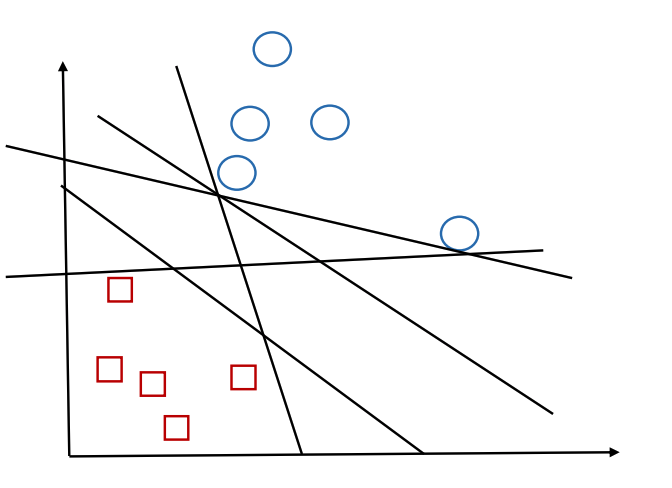
\includegraphics[scale=3]{picture/separating-lines.png}
    \caption{超平面}
    \label{separating_lines}
\end{figure}

为了选择一个分类效果最佳的超平面,支持向量机将距离超平面最近的点设定为支持向量,然后让这些支持向量和超平面
直接的距离最大,从而选择出一个最优的超平面,如图所示。并且对于线性分类不适用的非线性数据(如文本数据),支持向量机利用
核函数的技巧,通过选择一个恰当的转换函数,将非线性数据映射到一个更高维的向量空间当中,让数据重新分布为线性可分的形式。
但是这种做法增加了算法复杂度,复杂的核函数会使算法的计算量成倍的提高,而且如何选择合适的核函数让数据线性可分也没有一个统一
的方法。

\section{基于神经网络的短文本分类方法}
传统文本分类方法虽然在篇章级的长文本上能够有较好的分类效果,
但是对于文本信息量较少的短文本来说,却难以发挥效用。基于统计的
特征提取方法会在训练时生成庞大的特征词库,使得文本特征向量的维度依然很高,一旦文本长度过短,
特征向量就会变为稀疏向量,即数据只集中在向量中的某几维上,其他维度都为零。
文本特征向量的稀疏性一直是短文本分类上最难以解决的问题之一,为了解决这个难题,学者们有必要
尝试引入新的概念与特征提取技术。

\subsection{短文本的分布式表示方法}
短文本的分布式表示方法也称为词向量表示法。
在神经网络与深度学习模型中,输入数据通常需要转化为矩阵的形式。对于自然语言处理任务,则需要
将文本中的词语表示为一个向量,从而让模型理解文本并进一步提取特征,完成分类任务。

One-hot Representation是词向量表示法最简单的实现方式,具体方法与前文中介绍的向量空间模型
大致相同,针对具体语料可以快速得到每个单词的词向量。但与向量空间模型一样,也存在维度过高与稀疏性的问题,
并且从词向量之中无法得到词语之间的关系,对短文本分类任务并不适用。

为了得到连续稠密的词向量,Hinton等人提出了一种称之为词嵌入(Word Embedding)的词向量实现方法。
该方法旨在根据语料库中词语的分布式属性,来量化与分类不同词语的语义相似度。
通过一系列转换函数,将词语从高纬度空间映射到一个维度相对较低的向量空间,表示为低维实数向量,
从而有效的解决了向量的稀疏问题。并且这种映射方法还保留了词语之间的关系,
即意思相近的词语它们产生的词向量也会在向量空间中彼此靠近。
\subsection{卷积神经网络}
\subsection{循环神经网络}
\subsection{注意力机制}